\section{Data and theory}
\label{sec:theory}

In this work, the photon content of the proton $x\gamma(x,Q)$ is
extracted from a PDF analysis based on the combine inclusive DIS
cross-section data from HERA~\cite{Abramowicz:2015mha} and
supplemented by the ATLAS measurements of the high-mass Drell-Yan
differential cross sections at $\sqrt{s}=8$ TeV~\cite{Aad:2016zzw}.
%
While the HERA data is the backbone of all recent PDF fits, providing
information on the quark/anti-quark and gluon content of the proton,
the high-mass Drell-Yan data provides a direct sensitivity to the
photon PDF.
%
As matter of fact, dilepton production at the Born level can arise
from either quark-antiquark $s$-channel scattering or from
photon-photon $t$- and $u$-channel scattering mediated by a lepton, as
shown in Fig.~\ref{fig:photoninduced} \textbf{(update the diagrams)}.

%%%%%%%%%%%%%%%%%%%%%%%%%%%%%%%%%%%%%%%%%%%%%%%%%%%%%%%%%%%%%%%%
\begin{figure}[t]
  \begin{center}
    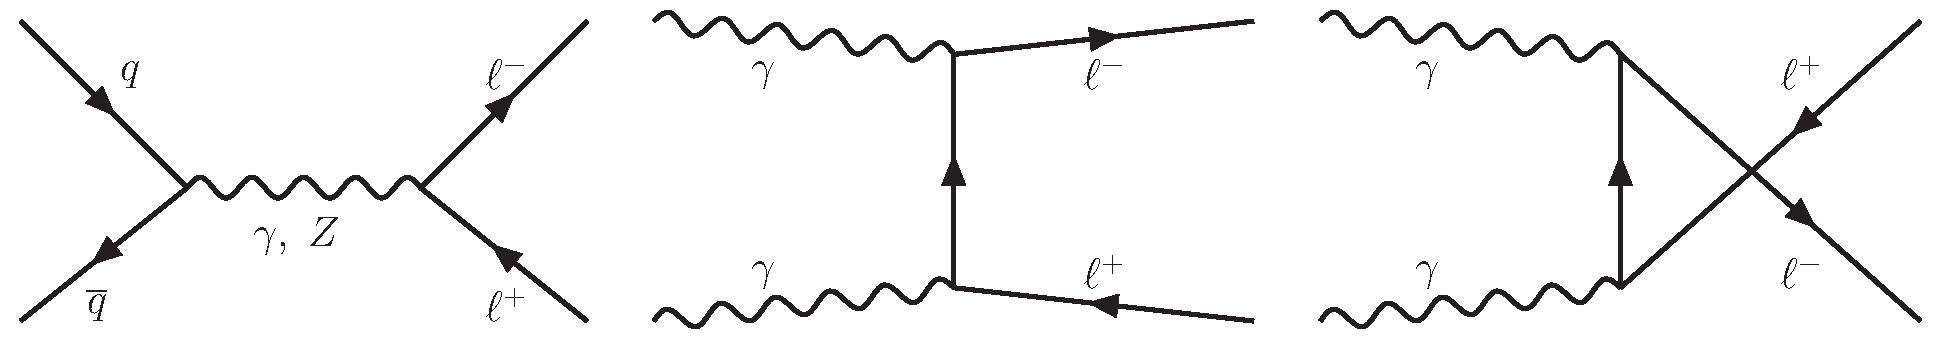
\includegraphics[width=17cm]{figs/DYdiagrams.pdf}
    \end{center}
    \caption{Diagrams that contribute to lepton-pair production at
      hadron colliders at the Born level.}
\label{fig:photoninduced}
\end{figure}
%%%%%%%%%%%%%%%%%%%%%%%%%%%%%%%%%%%%%%%%%%%%%%%%%%%%%%%%%%%%%%%%

DIS structure functions and PDF evolution are computed with the {\tt
  APFEL} program~\cite{Bertone:2013vaa}, which is currently accurate
up to NNLO in pure QCD and NLO in QED, and includes the relevant mixed
QCD+QED corrections. This means that, on top of the pure QCD
contributions, the DGLAP evolution
equations~\cite{Gribov:1972ri,Dokshitzer:1977,Altarelli:1977zs} are
solved including the $\mathcal{O}\lp \alpha_s\alpha\rp$ and
$\mathcal{O}\lp \alpha^2\rp$ corrections to the splitting functions.

As far as the DIS structure functions are concerned, corrections of
$\mathcal{O}\lp \alpha\rp$ are also included which in turn lead to an
explicit dependence of the predictions on the photon PDF.  The details
on the implementation as well as a discussion on the impact of these
corrections are given in appendix~\ref{sec:appendixAPFEL}.

Heavy-quark (charm and bottom) mass effects to DIS structure functions
are taken into account using the FONLL-B(C) general-mass
scheme~\cite{Forte:2010ta} for the NLO (NNLO) fits.
%
As for the numerical values of the heavy-quark masses in the pole-mass
scheme, we take $m_c=1.47~$GeV and $m_b=4.5~$GeV as determined in \cite{Abramowicz:2015mha}, which is also 
consistent with the latest PDG averages~\cite{Agashe:2014kda}.
%
The reference values of the coupling constants are chosen to be
$\alpha_s(m_Z)=0.118$ and $\alpha(m_\tau=1.777\mbox{ GeV})=1/133.4$.

For the calculation of high-mass Drell-Yan cross sections, we use the
{\tt MadGraph5{\_}aMC@NLO}~\cite{Alwall:2014hca} program v2.4.3, which
includes the contribution from photon-initiated diagrams, interfaced
to {\tt APPLgrid}~\cite{Carli:2010rw} v1.4.7 through {\tt
  aMCfast}~\cite{amcfast} v1.3).
%
A tailored version of {\tt APPLgrid} is used, allowing to account for
the contribution of the photon-initiated processes \footnote{Modified version of APPLgrid available at: $https://github.com/scarrazza/applgridphoton$}.
%
The calculation is performed in the $n_f=5$ scheme neglecting mass
effects of charm and bottom quarks in the matrix elements, as
appropriate for a high-scale processes.

The kinematic phase-space coverage of the data is presented in Fig.~\ref{fig:data}.
%%%%%%%%%%%%%%%%%%%%%%%%%%%%%%%%%%%%%%%%%%%%%%%%%%%%%%%%%%%%%%%%                                                                  
\begin{figure}[t]
  \begin{center}
    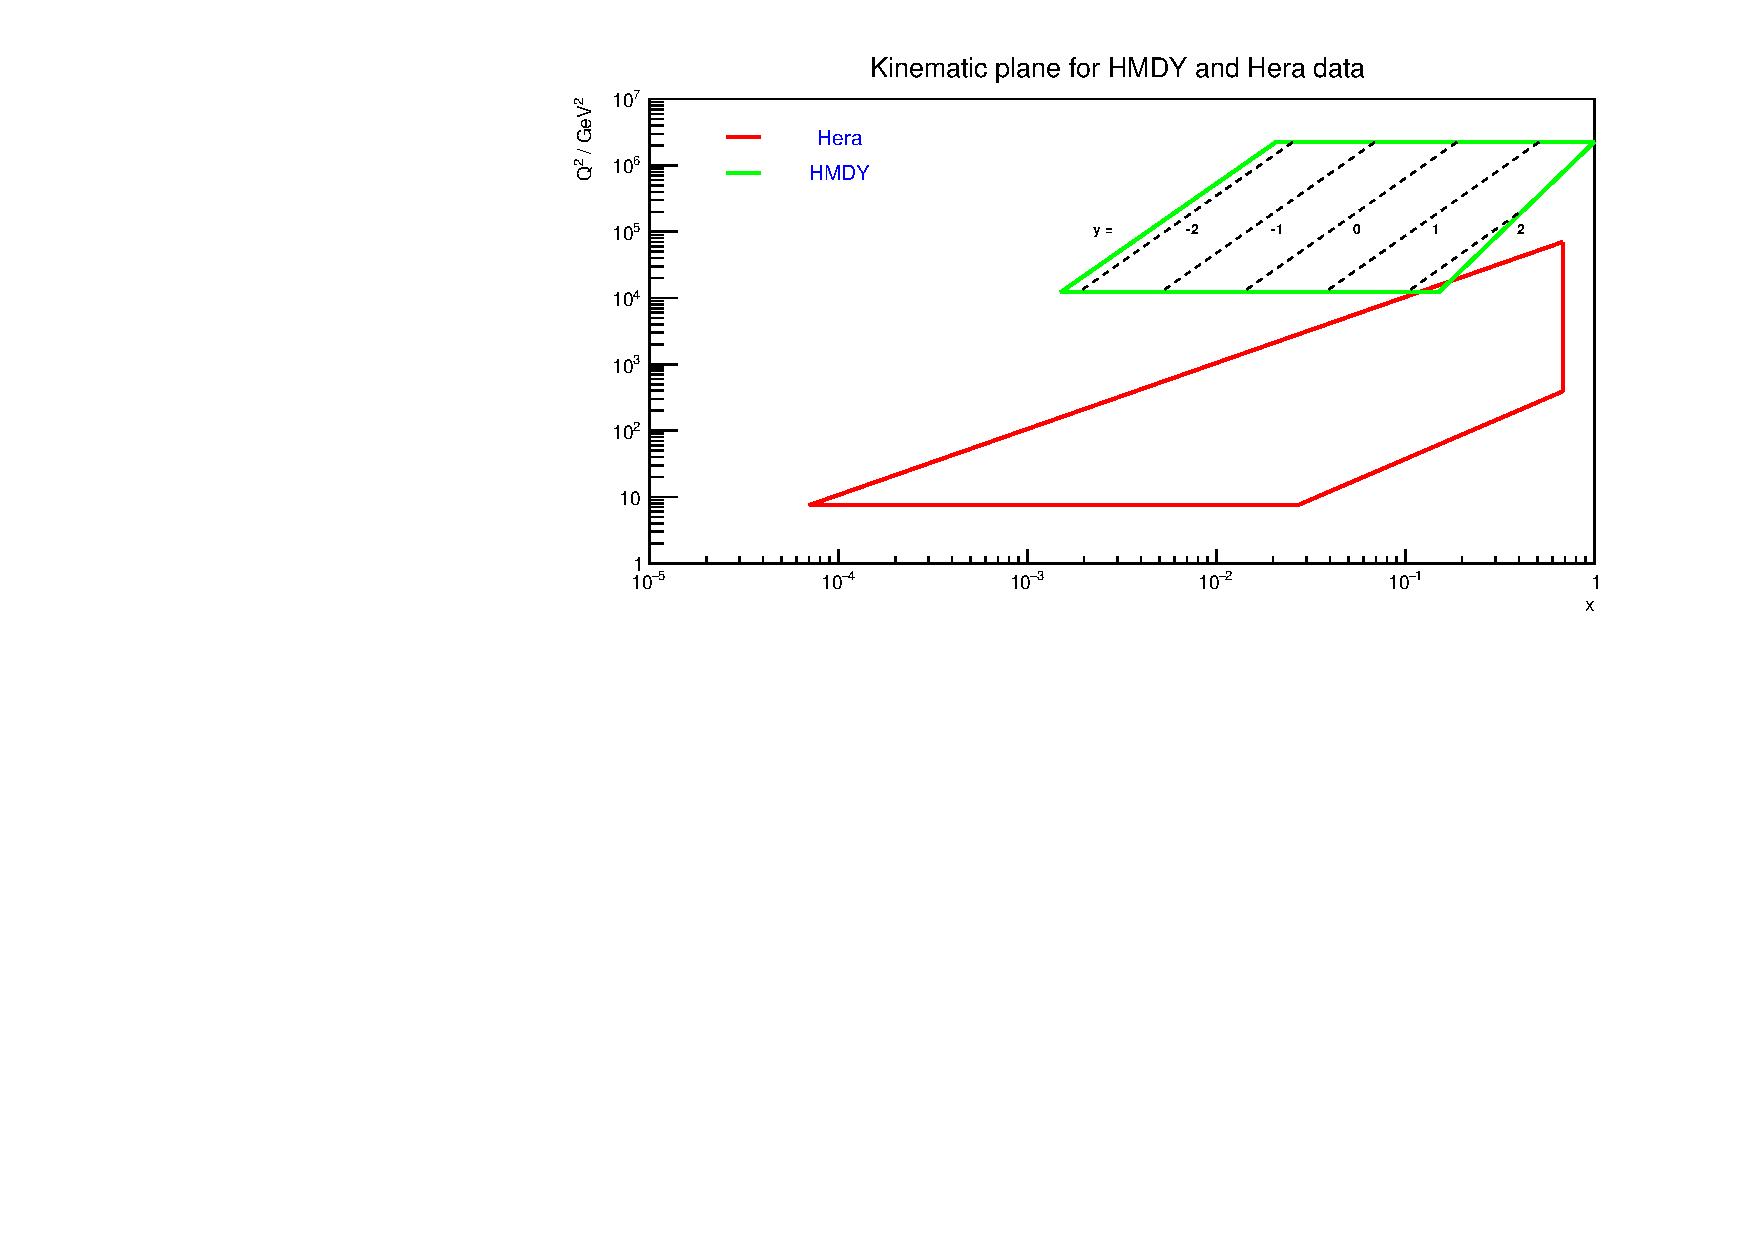
\includegraphics[width=10cm]{figs/kin2.pdf}
    \end{center}
    \caption{Kinematic coverage in $x$ and $Q^2$ plane of data used in this analysis: in red the HERA data, in green the high-mass DY data.}
\label{fig:data}
\end{figure}
%%%%%%%%%%%%%%%%%%%%%%%%%%%%%%%%%%%%%%%%%%%%%%%%%%%%%%%%%%%%%%%%      
The ATLAS high-mass Drell-Yan 8 TeV measurements include both the
single-differential (1D) invariant-mass distribution,
$d\sigma/dm_{ll}$, as well as the double-differential (2D)
distributions in $m_{ll}$ and $y_{ll}$,
$d^{2}\sigma/dm_{ll}d|y_{ll}|$, and in $m_{ll}$ and $\Delta\eta_{ll}$,
$d^{2}\sigma/dm_{ll}\Delta\eta_{ll}$.
%
For the invariant-mass distribution, there are 12 bins between 116 GeV
and 1.5 TeV; and for both of the double-differential distributions,
there are five different histograms, one for each of the different
invariant mass ranges, from the lowest bin with 116 GeV < $m_{ll}$ <
150 GeV to the highest bin with 500 GeV < $m_{ll}$ < 1500 GeV.
 %
The first three (last two) $m_{ll}$ bins are divided into 12 (6) bins
with fixed width, extending up to 2.4 and 3.0 for the $|y_{ll}^{mim}|$
and $|\Delta\eta_{ll}|$ distributions, respectively.
%
In Sect.~\ref{sec:results} we compare the impact on the photon PDF of
fitting either the 1D distributions or one of the two 2D
distributions.

In the theoretical calculations of the Drell-Yan cross section we use
dynamical renormalisation $\mu_{R}$ and factorisation $\mu_{R}$
scales, both set equal to the invariant mass $m_{ll}$ of the
respective bin.
%
The theoretical predictions for these measurements implement the
analysis cuts, including $m_{ll}\ge 116$ GeV, $\eta_l\le 2.5$,
$p_T^l \ge 40$ GeV$~(30)$ GeV for the leading (sub-leading) lepton.
%
The {\tt MadGraph5{\_}aMC@NLO} calculations used in this work were
benchmarked against the corresponding predictions (NLO QCD and LO QED,
including photon-induced processes) obtained with the {\tt FEWZ}
code~\cite{Gavin:2012sy} v3.1, finding agreement at the 1\% level or
better for both the 1D and the 2D distributions.
%
In order to achieve NNLO QCD and NLO EW accuracy in our theoretical
calculations, the NLO QCD + LO QED {\tt APPLgrid} tables generated
with {\tt aMCfast} have been supplemented by bin-by-bin $K$-factors,
defined as:
\begin{equation}
  \label{eq:kfactor}
  K \equiv\frac{\rm NNLO\  QCD  + NLO\  EW}{\rm NLO\  QCD + LO\  EW} \, ,
\end{equation}
using the MMHT2014 NNLO~\cite{Harland-Lang:2014zoa} PDF set both in
the numerator and in the denominator (NNLO $K$-factors depend very
mildly on the PDF set).
 %
The $K$-factors in Eq.~({\ref{eq:kfactor}) have been computed using
  the {\tt FEWZ} program, with the same settings as the corresponding
  NLO computations.
%

  In Fig.~\ref{fig:kf} we show the $K$-factors corresponding to the
  measurements included in our fits as a function of the dilepton
  rapidity $|y_{ll}|$, where each curve corresponds to a different
  dilepton invariant-mass $m_{ll}$ bin.
%
  We observe that the $K$-factors vary between 0.98 and 1.04,
  highlighting the fact that higher-order corrections to the Drell-Yan
  process are moderate, in particular at low values of $m_{ll}$ and in
  the central region.
%
  Even at forward rapidities, the $K$-factors modify the NLO result by
  at most 3\%.

%%%%%%%%%%%%%%%%%%%%%%%%%%%%%%%%%%%%%%%%%%%%%%%%%%%%%%%%
\begin{figure}[t]
\includegraphics[width=9cm]{figs/kf_2D.pdf}
\caption{The NNLO/NLO $K$-factors, defined in Eq.~(\ref{eq:kfactor}),
  that allow accounting for higher order QCD and EW effects in the PDF
  fits, as a function of the dilepton rapidity $|y_{ll}|$.  Each curve
  correspond to one of the $m_{ll}$ invariant mass bins.}
\label{fig:kf}
\end{figure}
%%%%%%%%%%%%%%%%%%%%%%%%%%%%%%%%%%%%%%%%%%%%%%%%%%%%%%%%
